% Scoring methodology. One sentence per line (clean diffs).
% Every number and rule is traced to code in notes/provenance.md.
\section{Spray-Exposure Scoring}
\label{sec:scoring}

A dishwasher can only clean a surface that its water reaches.
We therefore rank arrangements by how much of their food-contact surface is geometrically reachable from the spray arms, a quantity we call \emph{spray exposure}.
The score is a deterministic, simulation-free function of the object poses.
It connects the surfaces to be cleaned to the spray sources by straight segments and measures the share that the load leaves unobstructed, in the spirit of ambient occlusion in rendering~\cite{zhukov1998ambient}.
In the benchmark it serves two roles: it is the objective from which goal arrangements are synthesized, and it is the quality measure of the open track.
It contains no model of fluid transport and is not a cleaning measurement (Sec.~\ref{sec:scoring-limits}).
We first fix notation (Sec.~\ref{sec:scoring-notation}) and model the surfaces to be cleaned (Secs.~\ref{sec:scoring-food}--\ref{sec:scoring-sampling}), the spray sources (Sec.~\ref{sec:scoring-sources}) and line-of-sight transport (Sec.~\ref{sec:scoring-visibility}).
We then define the scores (Sec.~\ref{sec:scoring-score}) and the drainage constraint (Sec.~\ref{sec:scoring-pooling}), and state their properties (Sec.~\ref{sec:scoring-properties}).

\subsection{Arrangements and Notation}
\label{sec:scoring-notation}

All quantities are expressed in the dishwasher frame (meters, $z$ up).
The appliance has the racks $\mathcal{R}=\{\text{lower},\text{upper},\text{basket}\}$, which are scored in their closed, pushed-in configuration.
An instance contains objects $o\in\mathcal{O}$ of kind $\kappa(o)\in\{\text{plate},\text{bowl},\text{cup}\}$.
Each kind has a triangulated visual mesh $\mathcal{M}_\kappa$ in its object frame, whose $z$ axis is the axis of revolution.
An \emph{arrangement} $X=\{(T_o,r_o)\}_{o\in\mathcal{O}_X}$ assigns every racked object $o\in\mathcal{O}_X\subseteq\mathcal{O}$ a pose $T_o=(R_o,\vt_o)\in\SE$ and a rack $r_o\in\mathcal{R}$.
Objects outside the racks, e.g., on the counter, are not part of $X$ and are not scored; we assume $\mathcal{O}_X\neq\emptyset$.
A point $\vx$ and a direction $\vn$ of the object frame map to $T_o\vx=R_o\vx+\vt_o$ and $R_o\vn$.
The \emph{occluder geometry} of $X$ is the wire geometry $\Occ_{\mathrm{app}}$ of both racks and the basket together with the posed visual mesh of every racked object, the scored object included:
\begin{equation}
\Occ(X)=\Occ_{\mathrm{app}}\cup\bigcup_{o\in\mathcal{O}_X}T_o\,\mathcal{M}_{\kappa(o)}.
\label{eq:occluders}
\end{equation}
The tub walls, door and cabinet are not part of $\Occ(X)$.

\subsection{Food-Contact Surfaces}
\label{sec:scoring-food}

Only surfaces that touch food need to be cleaned.
Let $\tau_1,\dots,\tau_m$ be the triangles of $\mathcal{M}_\kappa$, with area $|\tau_i|$, centroid $\vc_i$ and unit normal $\vn_i$ oriented by the mesh winding toward free space.
Let $\hat{\vect{r}}_i=(c_{i,x},c_{i,y},0)^\top/\lVert(c_{i,x},c_{i,y})\rVert$ be the radial unit vector ($\hat{\vect{r}}_i=\vect{0}$ on the axis) and $z^{\mathrm{foot}}_\kappa=\min_{\vx\in\mathcal{M}_\kappa}x_z$ the foot height.
The food-contact surface of kind $\kappa$ is
\begin{align}
\mathcal{F}_\kappa&=\bigl\{\tau_i:\ \iota_i\ \land\ c_{i,z}>z^{\mathrm{foot}}_\kappa+\delta_f\bigr\},\label{eq:food}\\
\iota_i&=\bigl(\vn_i^\top\hat{\vect{r}}_i<-\alpha\bigr)\lor\bigl(n_{i,z}>\beta\bigr),\nonumber
\end{align}
with $\alpha=0.1$, $\beta=0.5$ and $\delta_f=3$\,mm.
The first test in $\iota_i$ keeps faces that look toward the axis, i.e., the inner wall of a bowl or cup.
The second keeps faces that look up: the top of a plate and the floor of a vessel.
The height test removes the inner wall of the foot ring, which also faces the axis.
Outer walls and undersides fail both tests, except the rim top and the upper part of the outer lip, which face up and are counted; they are a small part of $\mathcal{F}_\kappa$.
The food-contact area is $A_\kappa=\sum_{\tau_i\in\mathcal{F}_\kappa}|\tau_i|$ (Table~\ref{tab:scoring-params}), and we write $A_o=A_{\kappa(o)}$.
For the drainage test of Sec.~\ref{sec:scoring-pooling} we also keep the interior vertex set $\mathcal{I}_\kappa$, the vertices of $\mathcal{F}_\kappa$, and its rim band, the vertices within $\delta_r$ of the top, which span the lip round-over:
\begin{equation}
\mathcal{B}_\kappa=\bigl\{\vx\in\mathcal{I}_\kappa:\ x_z\ge\max_{\vy\in\mathcal{I}_\kappa}y_z-\delta_r\bigr\},\qquad\delta_r=1\,\text{mm}.
\label{eq:rim}
\end{equation}

\begin{table}[t]
\caption{Scoring Parameters}
\label{tab:scoring-params}
\centering
\footnotesize
\setlength{\tabcolsep}{3pt}
\begin{tabular}{@{}llp{3.3cm}c@{}}
\toprule
Symbol & Value & Meaning & Prov.\\
\midrule
$N$ & 500 & samples per object & D\\
$K$ & 64 & source points per disc & D\\
$\epsilon$ & 0.1\,mm & segment start offset along $\vn_j$ & D\\
$\alpha$, $\beta$ & 0.1, 0.5 & inward and upward normal thresholds in~\eqref{eq:food} & D\\
$\delta_f$ & 3\,mm & foot exclusion height & D\\
$\delta_r$ & 1\,mm & rim band & D\\
$\delta_p$ & 2\,mm & pooling tolerance & D\\
$\vc_{\mathrm{low}}$ & $(0,\,0.008,\,0.185)$\,m & lower-arm disc center (lower rack, basket) & A\\
$\rho_{\mathrm{low}}$ & 0.233\,m & lower-arm disc radius & A\\
$\vc_{\mathrm{mid}}$ & $(0,\,0.008,\,0.540)$\,m & middle-arm disc center (upper rack) & A\\
$\rho_{\mathrm{mid}}$ & 0.191\,m & middle-arm disc radius & A\\
$w_c$ & 0 & ceiling-nozzle weight (upper rack) & A\\
$A_\kappa$ & 502\,/\,340\,/\,215\,cm$^2$ & food-contact area of plate / bowl / cup & C\\
\bottomrule
\end{tabular}

\vspace{3pt}
{\footnotesize Prov.: D = design choice; A = modeling assumption; C = computed from the meshes.\par}
\end{table}

\subsection{Surface Sampling}
\label{sec:scoring-sampling}

Integrals over $\mathcal{F}_\kappa$ are approximated with $N$ samples placed by systematic sampling on the cumulative-area distribution~\cite{cochran1977sampling}, without random numbers.
Let $\tau'_1,\dots,\tau'_M$ be the triangles of $\mathcal{F}_\kappa$ in mesh order, let $C_i=\sum_{l\le i}|\tau'_l|/A_\kappa$ and, for $j=1,\dots,N$,
\begin{equation}
i(j)=\min\bigl\{\,i:\ C_i\ge (j-\tfrac12)/N\,\bigr\}.
\label{eq:sampling}
\end{equation}
Sample $j$ is the centroid $\bar{\vp}_j$ of $\tau'_{i(j)}$, with that triangle's normal $\bar{\vn}_j$, and represents the area $A_\kappa/N$.
Because the thresholds $(j-\frac12)/N$ are evenly spaced, triangle $\tau'_i$ receives $\lfloor N|\tau'_i|/A_\kappa\rfloor$ or $\lceil N|\tau'_i|/A_\kappa\rceil$ samples.
Our meshes have about $10^4$ food-contact triangles against $N=500$ samples, so most triangles receive none.
The rule therefore acts as a systematic sample along the ring-by-ring mesh order rather than a per-triangle quadrature.
For integrands that vary smoothly over the surface, $(A_\kappa/N)\sum_j f(\bar{\vp}_j)$ approximates $\int_{\mathcal{F}_\kappa}f\,\mathrm{d}A$ closely; for discontinuous integrands such as visibility the error is larger.
For object $o$ the samples are posed as $\vp_j=T_o\bar{\vp}_j$ and $\vn_j=R_o\bar{\vn}_j$ for $j\in\mathcal{S}_o$, $|\mathcal{S}_o|=N$.

\subsection{Spray Source Model}
\label{sec:scoring-sources}

A rotating spray arm sweeps a disc below its rack.
We replace each arm $a$ by its swept disc $\mathcal{D}_a$, which is horizontal with center $\vc_a$ and radius $\rho_a$.
Every rack is served by one arm: $\sigma(\text{lower})=\sigma(\text{basket})=\text{lower arm}$, and $\sigma(\text{upper})=\text{middle arm}$, the arm mounted beneath the upper rack.
The disc is discretized by the $K$ points of an equal-area Fibonacci (sunflower) lattice~\cite{vogel1979sunflower},
\begin{equation}
\vq_k=\vc_a+\rho_a\sqrt{(k+\tfrac12)/K}\,\bigl(\cos k\phi,\ \sin k\phi,\ 0\bigr)^\top,
\label{eq:sunflower}
\end{equation}
for $k=0,\dots,K-1$, with the golden angle $\phi=\pi(3-\sqrt5)$ and uniform weights $u_k=1/K$.
Point $k$ lies at the area-median radius of the $k$-th of $K$ concentric annuli of equal area $\pi\rho_a^2/K$, so in the coordinate $r^2$ the radii follow the midpoint rule.
The golden-angle azimuths make the set an equal-weight, low-discrepancy point set on $\mathcal{D}_a$, which uniform weights match to the uniform area measure; it is not a two-dimensional midpoint rule and carries no midpoint error bound for integrands that vary in azimuth.
The disc parameters (Table~\ref{tab:scoring-params}) follow the appliance model.
The centers sit between the tub floor ($0.152$\,m) and the lower-rack floor ($0.215$\,m), and just below the upper-rack floor (about $0.572$\,m).
Each radius is the measured half-width of its rack ($0.2625$\,m and $0.240$\,m) minus a margin ($29.5$\,mm and $49$\,mm).
These values are modeling assumptions, not measurements of the arms.
For upper-rack objects the model admits an extra source point at a ceiling nozzle with weight $w_c$, which rescales that rack's disc weights to $(1-w_c)/K$; we set $w_c=0$ because the nozzle has not been inspected.

\subsection{Line of Sight and Impingement}
\label{sec:scoring-visibility}

Consider a sample $j$ of object $o$ and a source point $\vq_k$ of the arm $\sigma(r_o)$.
Let $\vs_j=\vp_j+\epsilon\,\vn_j$ be the sample lifted off its own surface by $\epsilon=0.1$\,mm, and define the segment length and direction
\begin{equation}
\ell_{jk}=\lVert\vq_k-\vs_j\rVert,\qquad \vd_{jk}=(\vq_k-\vs_j)/\ell_{jk}.
\label{eq:segment}
\end{equation}
The segment is \emph{open} if it meets no occluder before reaching the source,
\begin{equation}
v_{jk}(X)=\ind\bigl[\{\vs_j+t\,\vd_{jk}:\ 0<t<\ell_{jk}\}\cap\Occ(X)=\emptyset\bigr],
\label{eq:visibility}
\end{equation}
and its \emph{impingement weight} is the cosine between the surface normal and the segment,
\begin{equation}
\gamma_{jk}=\max\bigl(0,\ \vn_j^\top\vd_{jk}\bigr).
\label{eq:cosine}
\end{equation}
A source point behind the tangent plane of the sample ($\gamma_{jk}=0$) cannot wet its face and drops out of the score.
Visibility is binary: a segment that grazes a single rack wire is blocked.
Because every segment ends at its source point, geometry beyond the disc plays no role, and no attenuation with distance is applied.
Fig.~\ref{fig:scoring}(a) illustrates the three cases.

\begin{figure}[t]
\centering
% Fig. scoring (a): one sample, its tangent plane, eight source points on the edge-on disc.
% Coordinates in cm, hand-computed: normal at -20 deg, so points with x > -0.6 are in front;
% the occluder (x = 1.4..1.6) blocks the segments to x = 1.9 and 2.6 at heights 0.647 and 1.1.
\begin{tikzpicture}[x=1cm,y=1cm,>={Stealth[length=4pt]},font=\footnotesize]
  % tangent plane of the sample
  \draw[gray,dashed] (-0.6,0) -- (0.542,3.14);
  % occluder: a neighboring dish seen edge-on
  \draw[fill=orange!25,draw=orange!60!black,rounded corners=1pt] (1.4,0.6) rectangle (1.6,3.0);
  \node[anchor=west,align=left] at (1.65,2.6) {neighboring\\dish};
  % segments behind the tangent plane (ignored)
  \foreach \x in {-2.6,-1.8,-1.0} \draw[gray!70,densely dotted,thick] (0.2,2.2) -- (\x,0);
  % open segments
  \foreach \x in {-0.3,0.4,1.1} \draw[blue!60!black,thick] (0.2,2.2) -- (\x,0);
  % blocked segments, drawn up to the hit
  \draw[red!70!black,thick,dashed] (0.2,2.2) -- (1.4,0.647);
  \draw[red!70!black,thick,dashed] (0.2,2.2) -- (1.4,1.1);
  \fill[red!70!black] (1.4,0.647) circle (1.3pt);
  \fill[red!70!black] (1.4,1.1) circle (1.3pt);
  % disc (edge-on) and its source points
  \draw[line width=1.6pt,blue!60!black] (-2.9,0) -- (2.9,0);
  \foreach \x in {-2.6,-1.8,-1.0,-0.3,0.4,1.1,1.9,2.6} \fill[blue!60!black] (\x,0) circle (1.6pt);
  \node[anchor=north] at (0,-0.08) {disc $\mathcal{D}_a$ (edge-on) with source points $\vq_k$};
  % surface patch, normal, sample
  \draw[line width=2.4pt,brown!70!black] (-0.074,1.448) -- (0.474,2.952);
  \draw[->,thick] (0.2,2.2) -- (1.046,1.892) node[anchor=south west,inner sep=1pt] {$\vn_j$};
  \fill (0.2,2.2) circle (1.5pt);
  \node[anchor=east] at (0.05,2.3) {$\vp_j$};
\end{tikzpicture}
\\[1pt]
{\footnotesize (a)}\\[6pt]
% Fig. scoring (b): drainage test on a hemispherical bowl profile (radius 0.9 cm), side view.
% Upright bowl = arc from 180 to 360 deg; a tilt of phi rotates it to 180+phi .. 360+phi.
% phi = 56: rim ends at 236 and 56 deg, bottom (270) is on the arc, so water fills the
%           circular segment below the chord at z = 0.9 sin(236) (from 236 to 304 deg).
% phi = 135: arc 315 .. 495 deg; its lowest point is the rim end at 315 deg, so it drains.
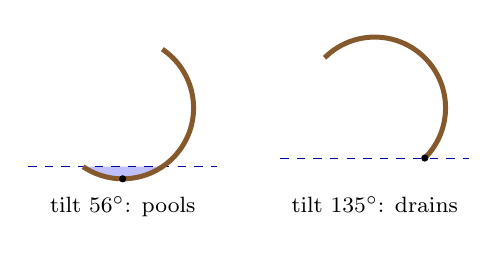
\begin{tikzpicture}[x=1cm,y=1cm,font=\footnotesize]
  \begin{scope}
    \fill[blue!25] (236:0.9) arc[start angle=236,end angle=304,radius=0.9] -- cycle;
    \draw[blue!60!black,dashed] (-1.2,{0.9*sin(236)}) -- (1.2,{0.9*sin(236)});
    \draw[line width=1.8pt,brown!70!black] (236:0.9) arc[start angle=236,end angle=416,radius=0.9];
    \fill (270:0.9) circle (1.3pt);
    \node[anchor=north,align=center] at (0,-1.0) {tilt $56^\circ$: pools};
  \end{scope}
  \begin{scope}[xshift=3.2cm]
    \draw[blue!60!black,dashed] (-1.2,{0.9*sin(315)}) -- (1.2,{0.9*sin(315)});
    \draw[line width=1.8pt,brown!70!black] (315:0.9) arc[start angle=315,end angle=495,radius=0.9];
    \fill (315:0.9) circle (1.3pt);
    \node[anchor=north,align=center] at (0,-1.0) {tilt $135^\circ$: drains};
  \end{scope}
\end{tikzpicture}
\\[1pt]
{\footnotesize (b)}
\caption{Scoring geometry (schematic, side view).
(a)~Sample $\vp_j$ with normal $\vn_j$ and source points $\vq_k$ on the edge-on disc.
Solid blue: open segments ($v_{jk}=1$).
Dashed red: segments blocked by a neighboring dish ($v_{jk}=0$).
Dotted gray: source points behind the tangent plane (dashed gray line), which are ignored ($\gamma_{jk}=0$).
Here $e_j$ is the cosine-weighted share of the five front-facing points that are open.
(b)~Drainage test~\eqref{eq:pool} on one bowl profile: tilted $56^\circ$ from upright, the lowest interior point lies below the water line through the lowest rim point and the bowl pools (shaded); tilted $135^\circ$ it drains.}
\label{fig:scoring}
\end{figure}

\subsection{Exposure Scores}
\label{sec:scoring-score}

\textit{Sample exposure:}
The exposure of sample $j$ is the impingement-weighted share of its front-facing source points that it sees unobstructed,
\begin{equation}
e_j(X)=
\begin{cases}
\dfrac{\sum_{k}u_k\,\gamma_{jk}\,v_{jk}(X)}{\sum_{k}u_k\,\gamma_{jk}}, & \text{if }\sum_{k}u_k\,\gamma_{jk}>0,\\[8pt]
0, & \text{otherwise.}
\end{cases}
\label{eq:sample-exposure}
\end{equation}
It discretizes the continuous exposure
\begin{equation}
e(\vp,\vn)=\frac{\int_{\mathcal{D}_a}\max\bigl(0,\vn^\top\vd(\vq)\bigr)\,V(\vp,\vq)\,\mathrm{d}A(\vq)}{\int_{\mathcal{D}_a}\max\bigl(0,\vn^\top\vd(\vq)\bigr)\,\mathrm{d}A(\vq)},
\label{eq:continuous}
\end{equation}
where $\vd(\vq)$ is the unit direction from $\vp$ to $\vq$, $V$ the binary visibility of~\eqref{eq:visibility}, and $\mathrm{d}A$ the uniform area measure on the disc.
Precisely,~\eqref{eq:sample-exposure} is the ratio of the $K$-point quadratures of the numerator and denominator of~\eqref{eq:continuous}.
It converges as $K\to\infty$ wherever the front-facing part of the disc has positive area; at finite $K$, a sample whose front-facing region contains no lattice point receives $e_j=0$.
Two design choices separate~\eqref{eq:continuous} from the irradiance $\int L_e\cos\theta_{\vp}\cos\theta_{\vq}\,V\,\lVert\vq-\vp\rVert^{-2}\,\mathrm{d}A$ that a uniform area emitter of radiance $L_e$ delivers, with both cosines clamped at zero~\cite{pharr2016pbrt}.
First, the emitter cosine and the inverse-square falloff are omitted: a geometric model cannot predict jet directions or intensities, so every point of the swept disc is treated as equally strong.
Second, the integral is normalized by its unoccluded value.
Hence, for a sample with at least one front-facing source point, $e_j=1$ exactly when none of them is blocked, however obliquely the surface faces the disc; $e_j$ then measures the occlusion caused by the load, the object itself included.
Samples with no front-facing source point score $0$, so $S$ also contains a hard orientation gate: an upward-facing food surface above its disc scores $0$ whatever the load, and $e_j$ jumps where the last front-facing source point crosses the tangent plane.

\textit{Object exposure:}
The exposure of object $o$ averages its samples,
\begin{equation}
E_o(X)=\frac1N\sum_{j\in\mathcal{S}_o}e_j(X)\ \approx\ \frac{1}{A_o}\int_{T_o\mathcal{F}_{\kappa(o)}}e\,\mathrm{d}A,
\label{eq:object-exposure}
\end{equation}
where the approximation follows from the area-proportional sampling of Sec.~\ref{sec:scoring-sampling}.

\textit{Arrangement score:}
The primary score is the area-weighted mean over the racked objects,
\begin{equation}
S(X)=\frac{\sum_{o\in\mathcal{O}_X}A_o\,E_o(X)}{\sum_{o\in\mathcal{O}_X}A_o}
=\frac{1}{A_X}\sum_{o\in\mathcal{O}_X}\sum_{j\in\mathcal{S}_o}\frac{A_o}{N}\,e_j(X),
\label{eq:score}
\end{equation}
with $A_X=\sum_{o\in\mathcal{O}_X}A_o$.
In the right-hand form every sample counts in proportion to the surface it represents, so $S$ estimates the mean exposure of all food-contact surface in the load.
A plate therefore weighs about as much as $1.5$ bowls or $2.3$ cups.
As a secondary, worst-case indicator we report $W(X)=\min_{o\in\mathcal{O}_X}E_o(X)$, which is not optimized.

\subsection{Drainage Constraint}
\label{sec:scoring-pooling}

An object that holds water after the wash is unacceptable whatever its exposure.
Object $o$ \emph{pools} in $X$ if its lowest interior vertex lies more than $\delta_p$ below the lowest point of its rim band,
\begin{equation}
\pool_o(X)\iff\min_{\vx\in\mathcal{I}_{\kappa(o)}}\bigl[T_o\vx\bigr]_z<\min_{\vx\in\mathcal{B}_{\kappa(o)}}\bigl[T_o\vx\bigr]_z-\delta_p,
\label{eq:pool}
\end{equation}
with $\delta_p=2$\,mm (Fig.~\ref{fig:scoring}(b)).
Water in a cavity can leave only over the rim, so it drains only if no interior point lies below the lowest point of the rim.
Our cavity profiles are convex below the lip, so~\eqref{eq:pool} decides drainage up to three tolerances: the mesh resolution, $\delta_p$, and the rim band, whose lowest point can lie slightly below the true spill crest because $\mathcal{B}_\kappa$ spans the lip round-over.
Puddles a few millimeters deep may therefore pass the test.
An arrangement is \emph{feasible} if no object pools, $\Phi(X)=\bigwedge_{o\in\mathcal{O}_X}\neg\pool_o(X)$.
Feasibility is a hard constraint rather than a penalty: the goal search accepts a change only if the resulting arrangement is feasible and raises $S$.
$S$ is computed in the same way for infeasible arrangements, and the feasibility of every scored load is reported beside $S$.

\subsection{Properties}
\label{sec:scoring-properties}

\begin{proposition}[Range and determinism]
\label{prop:range}
For every arrangement $X$ with $\mathcal{O}_X\neq\emptyset$, $e_j(X)$, $E_o(X)$, $S(X)$ and $W(X)$ lie in $[0,1]$, and all four are deterministic functions of $X$.
\end{proposition}
\noindent\textit{Proof:}
Since $0\le v_{jk}\le1$ and $u_k\gamma_{jk}\ge0$, the numerator of~\eqref{eq:sample-exposure} lies between $0$ and the denominator.
$E_o$, $S$ and $W$ are means, weighted means with positive weights, and minima of values in $[0,1]$.
No quantity in~\eqref{eq:occluders}--\eqref{eq:score} is random.\hfill$\square$

In floating point, identical inputs on a given device produce identical scores, and CPU and GPU agree to about $10^{-6}$ (Sec.~\ref{sec:scoring-impl}).

\begin{proposition}[Occlusion monotonicity]
\label{prop:monotone}
Let $X\subseteq X'$ be arrangements that assign the same poses and racks to the objects of $X$.
Then $E_o(X')\le E_o(X)$ for every $o\in\mathcal{O}_X$.
\end{proposition}
\noindent\textit{Proof:}
For $j\in\mathcal{S}_o$, the denominator of~\eqref{eq:sample-exposure} depends only on $\vp_j$, $\vn_j$ and the source points of $\sigma(r_o)$, which coincide in $X$ and $X'$.
By~\eqref{eq:occluders}, $\Occ(X)\subseteq\Occ(X')$, so every segment that is open in $X'$ is open in $X$, i.e., $v_{jk}(X')\le v_{jk}(X)$.
Hence $e_j(X')\le e_j(X)$ for all $j\in\mathcal{S}_o$, and averaging gives the claim.\hfill$\square$

Adding an object can thus only shade the objects already present.
The arrangement score, in contrast, is not monotone: adding an object whose exposure is below $S(X)$ lowers $S$ even if it shades nothing, and removing a poorly exposed object raises $S$.
We therefore compare $S$ only between complete loads of the same object set; a partial load is never a valid competitor.

\begin{remark}[Arm separability]
\label{rem:separable}
Let $z=z_{\mathrm{mid}}$ be the plane of the middle-arm disc.
If every lower-rack and basket object lies strictly below this plane and every upper-rack object strictly above it, then no object occludes a sample served by the other arm.
$S$ is then the area-weighted mean of two per-arm scores, one for the lower rack and basket together and one for the upper rack, each depending only on the poses of the objects its arm serves.
\end{remark}
\noindent This holds because an upper-rack segment joins a sample above the plane to a point on it, so it stays in the closed half-space $z\ge z_{\mathrm{mid}}$, which contains no lower-rack or basket object.
A lower-rack or basket segment joins a sample below the plane to a point of the lower disc, which also lies below it ($0.185<0.540$\,m), so it stays strictly below the plane, where there is no upper-rack object.
With the rack assignment fixed, so that the area weights stay constant, and the condition maintained, a planner may improve the two groups independently.

\subsection{Implementation}
\label{sec:scoring-impl}

We use $N=500$ samples per object and $K=64$ points per disc, i.e., $NK=32{,}000$ segment queries per object.
The occluders of $X$ are merged into one triangle set, indexed by the bounding-volume hierarchy of NVIDIA Warp~\cite{macklin2022warp}, and every segment is tested by a ray query whose maximum distance is $\ell_{jk}$.
The queries run on the GPU when one is available and on the CPU otherwise; the two agree to about $10^{-6}$, and we report scores to three decimals.
Two cheaper quantities support the benchmark without entering any reported goal or final value of $S$.
Candidate poses in the goal search are pre-ranked by the exposure of the candidate alone against the rack and basket wires, with no dishes and no self-occlusion ($N=200$, $K=32$).
Per-move score traces are $S$ evaluated at $N=120$, $K=32$ and are labeled as such.
Table~\ref{tab:scoring-params} lists every parameter with its provenance.

\subsection{Scope and Limitations}
\label{sec:scoring-limits}

$S$ is a line-of-sight proxy.
It contains no model of jets, splashing, sheeting, detergent or temperature, and it is not a measurement of cleaning.
The source discs, their placement and the uniform, distance-free weighting are modeling assumptions, and within a disc the score cannot tell where the jets actually point.
The food-contact and drainage rules are geometric and have not been validated against wash trials.
Because $S$ averages over the objects present, it ranks arrangements of the same object set only; values for different sets, such as different benchmark tiers, are not comparable.
